% !TeX program = xelatex
\documentclass[11pt,a4paper,landscape]{article}
\usepackage[margin=12mm]{geometry}
\usepackage{graphicx}
\usepackage[table]{xcolor}
\usepackage{array,tabularx}
\pagestyle{empty}
\setlength{\parindent}{0pt}
\setlength{\tabcolsep}{5pt}
\renewcommand{\arraystretch}{1.32}
\newcommand{\bomhead}{\rowcolor[gray]{.82}\textbf{Name} & \textbf{Number}\\\hline}
\newcommand{\category}[1]{\vspace{4mm}{\bfseries #1}\par\vspace{2mm}}
\begin{document}
{\LARGE BOM of each \textbf{Finger}}\par
\vspace{4mm}\hrule\vspace{5mm}
\begin{minipage}[t]{.30\textwidth}
\vspace{0pt}
\category{Electronic Devices}
\begin{tabularx}{\linewidth}{|X|c|}\hline
\bomhead
Motor & 1\\\hline
Camera & 1\\\hline
\end{tabularx}
\end{minipage}\hfill
\begin{minipage}[t]{.30\textwidth}
\vspace{0pt}
\category{3D Printed Parts}
\begin{tabularx}{\linewidth}{|X|c|}\hline
\bomhead
F1 (Right shell) & 1\\\hline
F2 (Left shell) & 1\\\hline
P1 (Idler pin) & 1\\\hline
\end{tabularx}
\end{minipage}\hfill
\begin{minipage}[t]{.34\textwidth}
\vspace{0pt}
\category{Mechanical Standard Parts}
\begin{tabularx}{\linewidth}{|X|c|}\hline
\bomhead
Screw M2$\times$4 & 8\\\hline
Screw M2.5$\times$12 & 2\\\hline
Screw M3$\times$6 & 1\\\hline
\end{tabularx}
\end{minipage}
\par\vspace{5mm}
% Original color exports. Scale is matched using the motor body in both views.
% Labels and leaders remain editable vector elements in the PDF.
\setlength{\unitlength}{1mm}
\begin{picture}(273,121)
\put(0,7){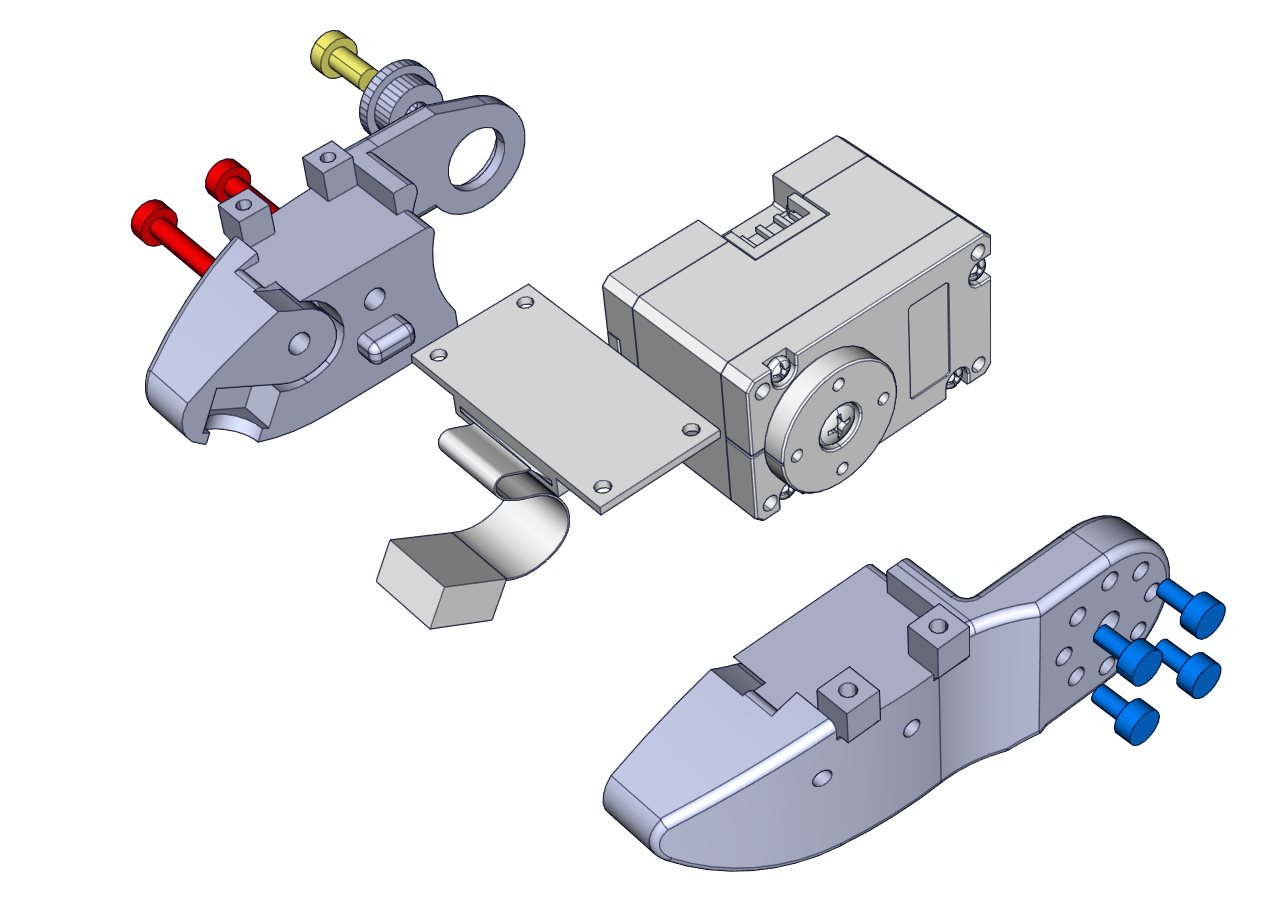
\includegraphics[width=150mm]{figures/finger_cam_exploded.jpg}}
\put(164,24){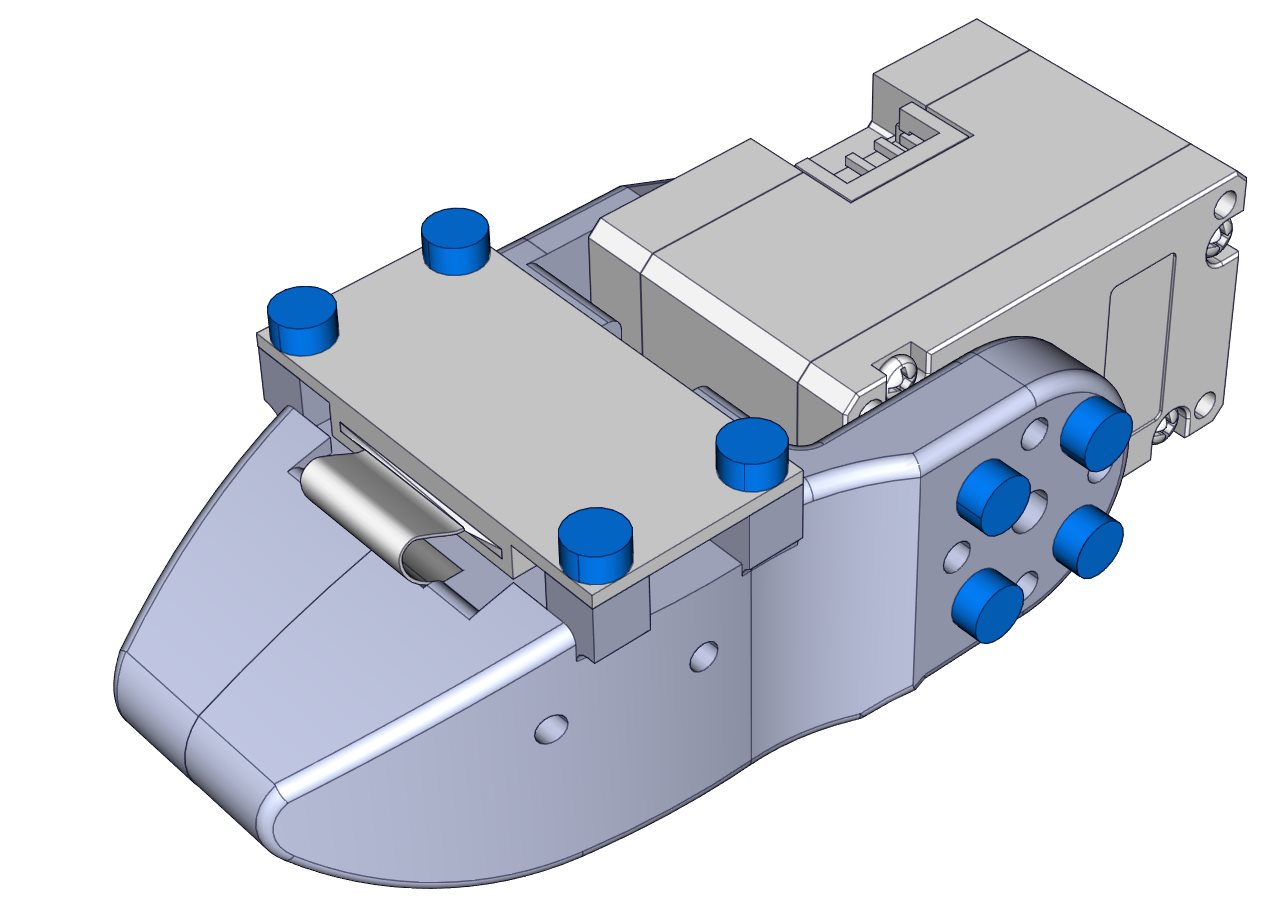
\includegraphics[width=102mm]{figures/finger_cam_closed.jpg}}
\thinlines\color{black}\small
% Exploded view: identifiers correspond to the printed-parts table.
\put(131,14){\circle{8}}\put(131,14){\makebox(0,0){F1}}
\qbezier(128,17)(118,27)(108,37)
\put(7,85){\circle{8}}\put(7,85){\makebox(0,0){F2}}
\qbezier(11,85)(25,84)(40,83)
\put(75,110){\circle{8}}\put(75,110){\makebox(0,0){P1}}
\qbezier(71.15,108.92)(58.075,105.26)(45,101.6)
% Fasteners exposed in the exploded view but hidden in the assembled view.
\put(3,105){\makebox(0,0)[l]{Screw M2.5$\times$12}}
\qbezier(20,102)(24,98)(28,92)
\put(63,117){\makebox(0,0)[l]{Screw M3$\times$6}}
\qbezier(66,114)(53,112)(40,109)
% Assembled view: device and visible fastener callouts.
\put(246,110){\makebox(0,0){Motor}}
\qbezier(246,107)(245,93)(244,80)
\put(171,99){\makebox(0,0){Camera}}
\qbezier(178,98)(193,80)(208,63)
\put(266,30){\makebox(0,0)[r]{Screw M2$\times$4}}
\qbezier(244,33)(245,47)(247,60)
\qbezier(244,33)(224,38)(210,52)
\put(76,0){\makebox(0,0){Exploded View}}
\put(215,0){\makebox(0,0){Assembled View}}
\end{picture}
\end{document}
